\documentclass[12pt,a4paper,openright,twoside]{book}
\usepackage[utf8]{inputenc}
\usepackage{disi-thesis}
\usepackage{code-lstlistings}
\usepackage{notes}
\usepackage{shortcuts}
\usepackage{acronym}
\usepackage{amsmath}
\usepackage{mathtools}

\school{\unibo}
\programme{Corso di Laurea
%[Magistrale?]
in Ingegneria e Scienze Informatiche}
\title{
%Fancy Title
Navigazione e Guida Autonoma di Veicoli Aerospaziali: Filtro di Kalman e sue varianti
}
\author{
%Candidate Name
Marco Buda
}
\date{\today}
\subject{
%Supervisor's course name
Metodi Numerici
}
\supervisor{Prof.ssa
%Supervisor Here
Damiana Lazzaro
}
%\cosupervisor{Dott. CoSupervisor 1}
%\morecosupervisor{Dott. CoSupervisor 2}
\session{
%I
II % TODO: verificare
}
\academicyear{
%2022-2023
2024-2025
}

% Definition of acronyms
\acrodef{IoT}{Internet of Thing}
\acrodef{vm}[VM]{Virtual Machine}


\mainlinespacing{1.241} % line spacing in mainmatter, comment to default (1)

\begin{document}

\frontmatter\frontispiece

\begin{abstract}	
Max 2000 characters, strict.
\end{abstract}

\begin{dedication} % this is optional
Optional. Max a few lines.
\end{dedication}

%----------------------------------------------------------------------------------------
\tableofcontents   
\listoffigures     % (optional) comment if empty
\lstlistoflistings % (optional) comment if empty
%----------------------------------------------------------------------------------------

\mainmatter

%----------------------------------------------------------------------------------------
\chapter{Introduction}
\label{chap:introduction}
%----------------------------------------------------------------------------------------

Write your intro here.
\sidenote{Add sidenotes in this way. They are named after the author of the thesis}

You can use acronyms that your defined previously,
such as \ac{IoT}.
%
If you use acronyms twice,
they will be written in full only once
(indeed, you can mention the \ac{IoT} now without it being fully explained).
%
In some cases, you may need a plural form of the acronym.
%
For instance,
that you are discussing \acp{vm},
you may need both \ac{vm} and \acp{vm}.

\paragraph{Structure of the Thesis}

\note{At the end, describe the structure of the paper}

\chapter{State of the art}

\section{I sistemi dinamici}

Un sistema dinamico è un qualunque sistema in cui sia individuabile uno stato che evolve come funzione del tempo: $x=f(t)$. \\
Per gli scopi di questa tesi, lo stato verrà rappresentato come un vettore $x\in\mathbb{R}^n$, che raccoglie le variabili di stato (es.: posizione, velocità...), e il tempo verrà considerato come una quantità continua $t\in\mathbb{R}$, eventualmente campionata in determinati istanti $t_k$.

Modellizzare la realtà a livello macroscopico comporta spesso che $f$ sia non deterministica, per via di fenomeni microscopici. Questo introduce la necessità di effettuare misurazioni periodiche (\textit{measurement}, $z\in\mathbb{R}^m$) per monitorare la reale evoluzione dello stato in presenza di disturbi (\textit{process noise}, $w\in\mathbb{R}^n$). \\
Sfortunatamente, le misurazioni stesse sono soggette ad ulteriori disturbi (\textit{measurement noise}, $v\in\mathbb{R}^m$). \\
Nasce, quindi, l'esigenza di algoritmi che raccolgano ed interpretino i dati misurati per determinare una stima (\textit{state estimate}, $\hat{x}$) dello stato reale (\textit{ground truth}, $x$). Questi algoritmi sono detti, appunto, stimatori.

\section{Il filtro di Kalman}

Il filtro di Kalman~\cite{10.1115/1.3662552} è uno stimatore lineare ricorsivo che minimizza l'errore quadratico medio. \\
L'aspetto ricorsivo si rifà al fatto che ogni stima $\hat{x}_k$ è determinata in base alla stima precedente $\hat{x}_{k-1}$ e alla misurazione attuale $z_k$, senza richiedere l'utilizzo esplicito di $\hat{x}_0,\hat{x}_1,...,\hat{x}_{k-2}$ o $z_0,...,z_{k-1}$. Si tratta di uno dei principali vantaggi del filtro, in quanto riduce sia la complessità temporale che quella spaziale, senza compromettere l'ottimalità. \\
Come anticipato, l'ottimalità è definita dal fatto che, ad ogni passo $k$, l'algoritmo produce la stima $\hat{x}_k$ che minimizza la quantità $\mathbb{E}[\lVert e_k\rVert^2]$, con $e_k=\hat{x}_k-x_k$. \\

\subsection{Definizione del problema lineare}

Il filtro di Kalman può essere applicato a sistemi dinamici che siano rappresentabili con un modello ricorsivo lineare:
\begin{equation}
x_k=A_kx_{k-1}+B_ku_{k-1}+w_{k-1}
\end{equation}
dove $A_k$ è la matrice $n\times n$ di evoluzione dello stato dal passo $k-1$ al passo $k$ in assenza di disturbi e ``azioni di controllo'', $B_k$ è la matrice $l\times n$ di contributo delle ``azioni di controllo'' (\textit{control input}, es.: forza di gravità, propulsione...) $u_{k-1}\in\mathbb{R}^l$ che agiscono dal passo $k-1$ al passo $k$ e $w_{k-1}\in\mathbb{R}^n$ è il \textit{process noise} che agisce dal passo $k-1$ al passo $k$. \\

In aggiunta, è richiesto che le misurazioni siano lineari rispetto allo stato:
\begin{equation}
z_k=H_kx_k+v_k
\end{equation}
dove $H_k$ è la matrice $m\times n$ che determina le variabili osservate in base allo stato che si vuole stimare e $v_k\in\mathbb{R}^m$ è il \textit{measurement noise}.
\pagebreak

Sono posti dei vincoli di non correlazione fra le variabili aleatorie:
\begin{gather*}
\mathrm{Cov}(w_k,u_j)=0_{n\times l},\quad\forall\,k,\forall\,0\leq j<k \\
\mathrm{Cov}(w_k,w_j)=0_{n\times n},\quad\forall\,k,\forall\,0\leq j<k \\
\mathrm{Cov}(w_k,v_j)=0_{n\times m},\quad\forall\,k,\forall\,1\leq j\leq k \\
\mathrm{Cov}(w_k,x_0)=0_{n\times n},\quad\forall\,k
\end{gather*}

Infine, nelle formulazioni standard del filtro, si richiede che $w$ e $v$ siano privi di \textit{bias}, ossia che $\mathbb{E}[w_k]=\underline{0}$ e $\mathbb{E}[v_k]=\underline{0}$, ad ogni passo $k$.

\subsection{Costruzione del filtro lineare}

Il primo passo è descrivere l'espressione che calcoli la stima $\hat{x}_k$. Al passo $k\geq 1$ sono disponibili le informazioni riguardo $\hat{x}_{k-1}$, $u_{k-1}$ e $z_k$, per cui l'espressione lineare avrà la forma generica:
\begin{equation*}
\hat{x}_k=\mathcal{A}_k\hat{x}_{k-1}+\mathcal{B}_ku_{k-1}+\mathcal{K}_kz_k
\end{equation*}
Per quanto riguarda il passo $k=0$, la scelta della stima iniziale $\hat{x}_0$ è libera, purché sia deterministica. Se si hanno informazioni sulla distribuzione di $x_0$, è consigliabile scegliere $\hat{x}_0=\mathbb{E}[x_0]$, o una sua stima. \\

Una condizione implicita sul filtro richiede che anche l'errore sulle stime generate $e_k$ sia privo di \textit{bias}, ossia, ad ogni passo $k$:
$$\mathbb{E}[e_k]=\mathbb{E}[\hat{x}_k-x_k]=\underline{0}$$
Da questa condizione si otterranno informazioni sulle matrici incognite $\mathcal{A}$, $\mathcal{B}$ e $\mathcal{K}$. In effetti, considerando per $k\geq 1$ e sostituendo $\hat{x}_k$ con la sua definizione, si ottiene:
$$\mathbb{E}[\mathcal{A}_k\hat{x}_{k-1}+\mathcal{B}_ku_{k-1}+\mathcal{K}_kz_k-x_k]=\underline{0}$$
Successivamente, sostituendo $z_k$ con la sua definizione:
$$\mathbb{E}\left[\mathcal{A}_k\hat{x}_{k-1}+\mathcal{B}_ku_{k-1}+\mathcal{K}_k\bigl(H_kx_k+v_k\bigr)-x_k\right]=\underline{0}$$
Sostituendo $x_k$ con la sua relazione ricorsiva e manipolando i termini:
\begin{gather*}
\begin{multlined}[\textwidth]
\mathbb{E}\Bigl[\mathcal{A}_k\hat{x}_{k-1}+\mathcal{B}_ku_{k-1}+\mathcal{K}_k\Bigl(H_k\bigl(A_kx_{k-1}+B_ku_{k-1}+w_{k-1}\bigr)+v_k\Bigr)+ \\
-\bigl(A_kx_{k-1}+B_ku_{k-1}+w_{k-1}\bigr)\Bigr]=\underline{0}
\end{multlined} \\
\begin{multlined}[\textwidth]
\Rightarrow\mathbb{E}\bigl[\mathcal{A}_k\hat{x}_{k-1}+\mathcal{B}_ku_{k-1}+\mathcal{K}_kH_kA_kx_{k-1}+\mathcal{K}_kH_kB_ku_{k-1}+\mathcal{K}_kH_kw_{k-1}+ \\
+\mathcal{K}_kv_k-A_kx_{k-1}-B_ku_{k-1}-w_{k-1}\bigr]=\underline{0}
\end{multlined} \\
\begin{multlined}[\textwidth]
\Rightarrow\mathbb{E}\bigl[\mathcal{A}_k\hat{x}_{k-1}+\mathcal{B}_ku_{k-1}+\mathcal{K}_kH_kA_kx_{k-1}+\mathcal{K}_kH_kB_ku_{k-1}+\mathcal{K}_kH_kw_{k-1}+ \\
+\mathcal{K}_kv_k-A_kx_{k-1}-B_ku_{k-1}-w_{k-1}-\mathcal{A}_kx_{k-1}+\mathcal{A}_kx_{k-1}\bigr]=\underline{0}
\end{multlined} \\
\begin{multlined}[\textwidth]
\Rightarrow\mathbb{E}\bigl[\mathcal{A}_k\bigl(\hat{x}_{k-1}-x_{k-1}\bigr)+\bigl(\mathcal{K}_kH_kA_k-A_k+\mathcal{A}_k\bigr)x_{k-1}+ \\
+\bigl(\mathcal{K}_kH_kB_k-B_k+\mathcal{B}_k\bigr)u_{k-1}+\bigl(\mathcal{K}_kH_k-I\bigr)w_{k-1}+\mathcal{K}_kv_k\bigr]=\underline{0}
\end{multlined} \\
\begin{multlined}[\textwidth]
\Rightarrow\mathcal{A}_k\mathbb{E}[\hat{x}_{k-1}-x_{k-1}]+\bigl(\mathcal{K}_kH_kA_k-A_k+\mathcal{A}_k\bigr)\mathbb{E}[x_{k-1}]+ \\
+\bigl(\mathcal{K}_kH_kB_k-B_k+\mathcal{B}_k\bigr)\mathbb{E}[u_{k-1}]+\bigl(\mathcal{K}_kH_k-I\bigr)\mathbb{E}[w_{k-1}]+\mathcal{K}_k\mathbb{E}[v_k]=\underline{0}
\end{multlined}
\end{gather*}
Sfruttando l'ipotesi che le quantità $\hat{x}_{k-1}-x_{k-1}$, $w_{k-1}$ e $v_k$ siano prive di \textit{bias}:
$$\bigl(\mathcal{K}_kH_kA_k-A_k+\mathcal{A}_k\bigr)\mathbb{E}[x_{k-1}]+\bigl(\mathcal{K}_kH_kB_k-B_k+\mathcal{B}_k\bigr)\mathbb{E}[u_{k-1}]=\underline{0}$$
Non potendo fare assunzioni su $x$ e $u$, ne segue che:
$$\mathcal{K}_kH_kA_k-A_k+\mathcal{A}_k=\underline{0}\enspace,\quad\mathcal{K}_kH_kB_k-B_k+\mathcal{B}_k=\underline{0}$$
$$\Rightarrow\mathcal{A}_k=(I-\mathcal{K}_kH_k)A_k\enspace,\quad\mathcal{B}_k=(I-\mathcal{K}_kH_k)B_k$$

Risulta pratico definire la seguente quantità come una stima \textit{a priori}, ossia che non tiene conto della misurazione al passo $k\geq 1$:
$$\hat{x}_k^-=A_k\hat{x}_{k-1}+B_ku_{k-1}$$
L'espressione per ricavare $\hat{x}_k$, ossia la stima \textit{a posteriori}, diventa, perciò:
$$\hat{x}_k=(I-\mathcal{K}_kH_k)A_k\hat{x}_{k-1}+(I-\mathcal{K}_kH_k)B_ku_{k-1}+\mathcal{K}_kz_k=$$
$$=(I-\mathcal{K}_kH_k)(A_k\hat{x}_{k-1}+B_ku_{k-1})+\mathcal{K}_kz_k=(I-\mathcal{K}_kH_k)\hat{x}_k^-+\mathcal{K}_kz_k=$$
$$=\hat{x}_k^-+\mathcal{K}_k(z_k-H_k\hat{x}_k^-)$$

Proseguendo, si definisca $e_k^-=\hat{x}_k^--x_k$ come l'errore sulla stima \textit{a priori} e si consideri:
$$e_k^-=\hat{x}_k^--x_k=(A_k\hat{x}_{k-1}+B_ku_{k-1})-(A_kx_{k-1}+B_ku_{k-1}+w_{k-1})=$$
$$=A_k(\hat{x}_{k-1}-x_{k-1})-w_{k-1}=A_ke_{k-1}-w_{k-1}$$
Si osservi che anche $e_k^-$ è privo di \textit{bias}:
$$\mathbb{E}[e_k^-]=\mathbb{E}[A_ke_{k-1}-w_{k-1}]=A_k\mathbb{E}[e_{k-1}]-E[w_{k-1}]=\underline{0}$$

Si definiscano, per $k\geq 1$, le auto-covarianze degli errori $P_k^-=\mathrm{Cov}(e_k^-,e_k^-)$ e $P_k=\mathrm{Cov}(e_k,e_k)$. \\
Si ha:
\begin{gather*}
P_k^-=\mathbb{E}\left[(e_k^--\mathbb{E}[e_k^-])(e_k^--\mathbb{E}[e_k^-])^T\right]=\mathbb{E}\left[e_k^-(e_k^-)^T\right]= \\
=\mathbb{E}\left[(A_ke_{k-1}-w_{k-1})(A_ke_{k-1}-w_{k-1})^T\right]= \\
=\mathbb{E}\left[(A_ke_{k-1}-w_{k-1})\left({e_{k-1}}^T{A_k}^T-{w_{k-1}}^T\right)\right]= \\
\begin{multlined}[\textwidth]
=A_k\mathbb{E}\left[e_{k-1}(e_{k-1})^T\right]{A_k}^T-A_k\mathbb{E}\left[e_{k-1}(w_{k-1})^T\right]+ \\
-\mathbb{E}\left[w_{k-1}(e_{k-1})^T\right]{A_k}^T+\mathbb{E}\left[w_{k-1}(w_{k-1})^T\right]=
\end{multlined} \\
\begin{multlined}[\textwidth]
=A_k\mathbb{E}\left[(e_{k-1}-\underline{0})(e_{k-1}-\underline{0})^T\right]{A_k}^T-A_k\mathbb{E}\left[(e_{k-1}-\underline{0})(w_{k-1}-\underline{0})^T\right]+ \\
-\mathbb{E}\left[(w_{k-1}-\underline{0})(e_{k-1}-\underline{0})^T\right]{A_k}^T+\mathbb{E}\left[(w_{k-1}-\underline{0})(w_{k-1}-\underline{0})^T\right]=
\end{multlined} \\
\begin{multlined}[\textwidth]
=A_k\mathbb{E}\left[(e_{k-1}-\mathbb{E}[e_{k-1}])(e_{k-1}-\mathbb{E}[e_{k-1}])^T\right]{A_k}^T+ \\
-A_k\mathbb{E}\left[(e_{k-1}-\mathbb{E}[e_{k-1}])(w_{k-1}-\mathbb{E}[w_{k-1}])^T\right]+ \\
-\mathbb{E}\left[(w_{k-1}-\mathbb{E}[w_{k-1}])(e_{k-1}-\mathbb{E}[e_{k-1}])^T\right]{A_k}^T+ \\
+\mathbb{E}\left[(w_{k-1}-\mathbb{E}[w_{k-1}])(w_{k-1}-\mathbb{E}[w_{k-1}])^T\right]=
\end{multlined} \\
\begin{multlined}[\textwidth]
=A_k\mathrm{Cov}(e_{k-1},e_{k-1}){A_k}^T-A_k\mathrm{Cov}(e_{k-1},w_{k-1})+ \\
-\mathrm{Cov}(w_{k-1},e_{k-1}){A_k}^T+\mathrm{Cov}(w_{k-1},w_{k-1})
\end{multlined}
\end{gather*}
Si osservi che i termini centrali si annullano se $e_{k-1}$ e $w_{k-1}$ sono non correlati. In effetti, analizzando ricorsivamente l'errore $e_{k-1}$, si trova che le uniche variabili aleatorie da cui esso dipende sono $u_0,...,u_{k-2}$, $w_0,...,w_{k-2}$, $v_1,...,v_{k-1}$ e $x_0$, ossia variabili con cui $w_{k-1}$ è non correlato per ipotesi. \\
Ricordando la definizione di $P_{k-1}$ e definendo $Q_{k-1}$ come la auto-covarianza di $w_{k-1}$, si trova, dunque, l'espressione:
$$P_k^-=A_kP_{k-1}{A_k}^T+Q_{k-1}$$
La scelta iniziale di $P_0$ è pressoché libera. Se si hanno informazioni sulla distribuzione di $x_0$, è consigliabile utilizzare una stima della sua auto-covarianza. In ogni caso, è necessario avere $P_0\neq 0_{n\times n}$ e semidefinita positiva.

I suggest referencing stuff as follows: \cref{fig:random-image} or \Cref{fig:random-image}

\begin{figure}
    \centering
    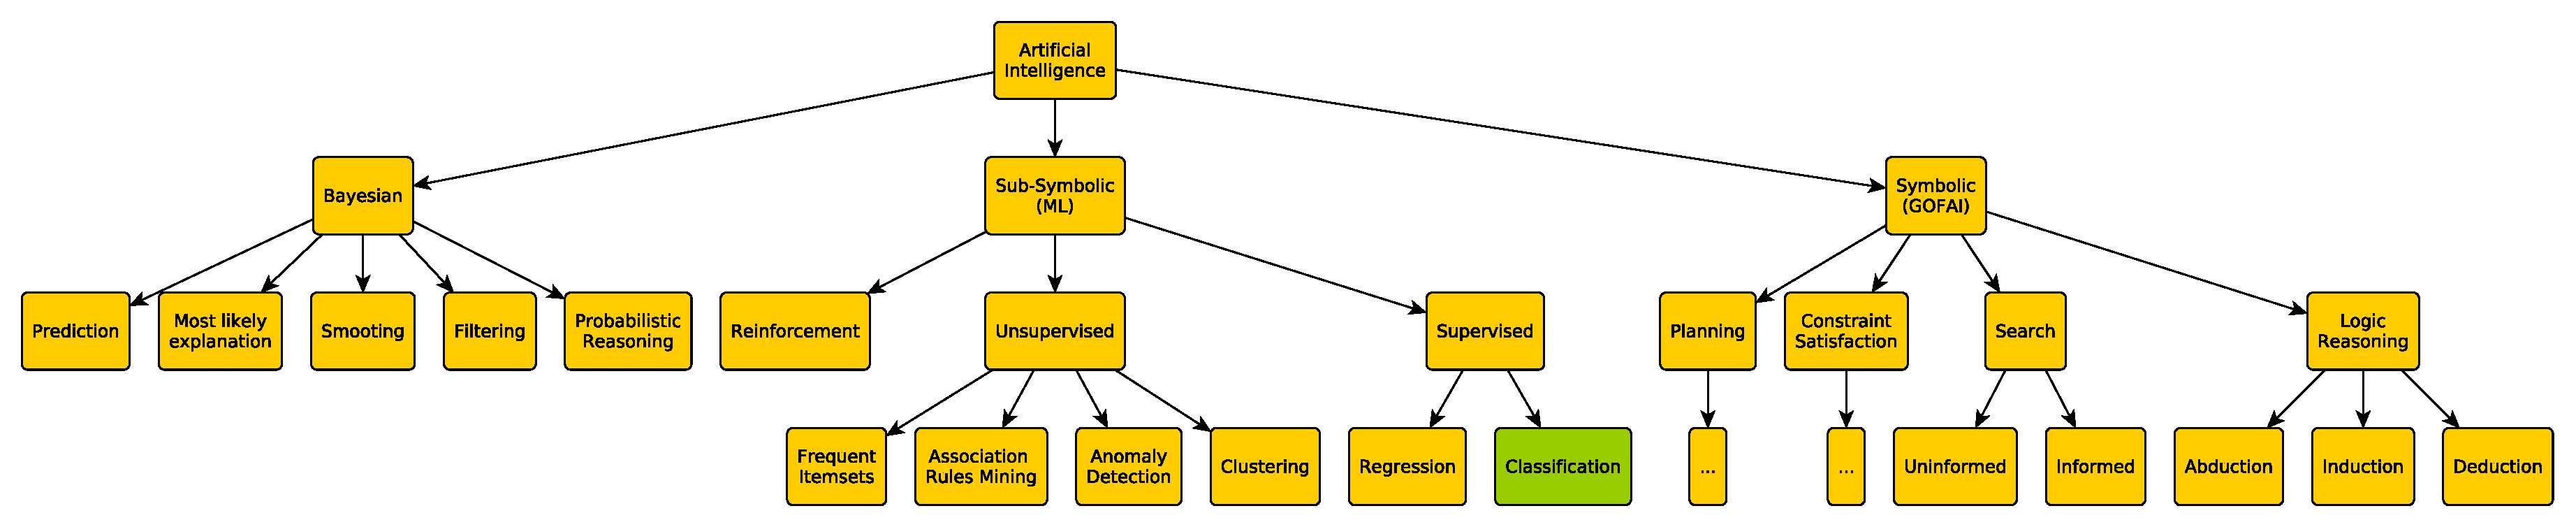
\includegraphics[width=.8\linewidth]{figures/random-image.pdf}
    \caption{Some random image}
    \label{fig:random-image}
\end{figure}

\section{Some cool topic}

\chapter{Contribution}

You may also put some code snippet (which is NOT float by default), eg: \cref{lst:random-code}.

\lstinputlisting[float,language=Java,label={lst:random-code}]{listings/HelloWorld.java}

\section{Fancy formulas here}

%----------------------------------------------------------------------------------------
% BIBLIOGRAPHY
%----------------------------------------------------------------------------------------

\backmatter

% \nocite{*} % Remove this as soon as you have the first citation

\bibliographystyle{alpha}
\bibliography{bibliography}

\begin{acknowledgements} % this is optional
Optional. Max 1 page.
\end{acknowledgements}

\end{document}
